\section{Synthesis and Implementation Results}

\subsection{Vivado Implementation Summary}

The Ring Flasher design was synthesized and implemented in Vivado on an Artix-7 FPGA. The post-implementation results are summarized below for an 8 ns clock period (125 MHz).

\begin{figure}[H]
    \centering
    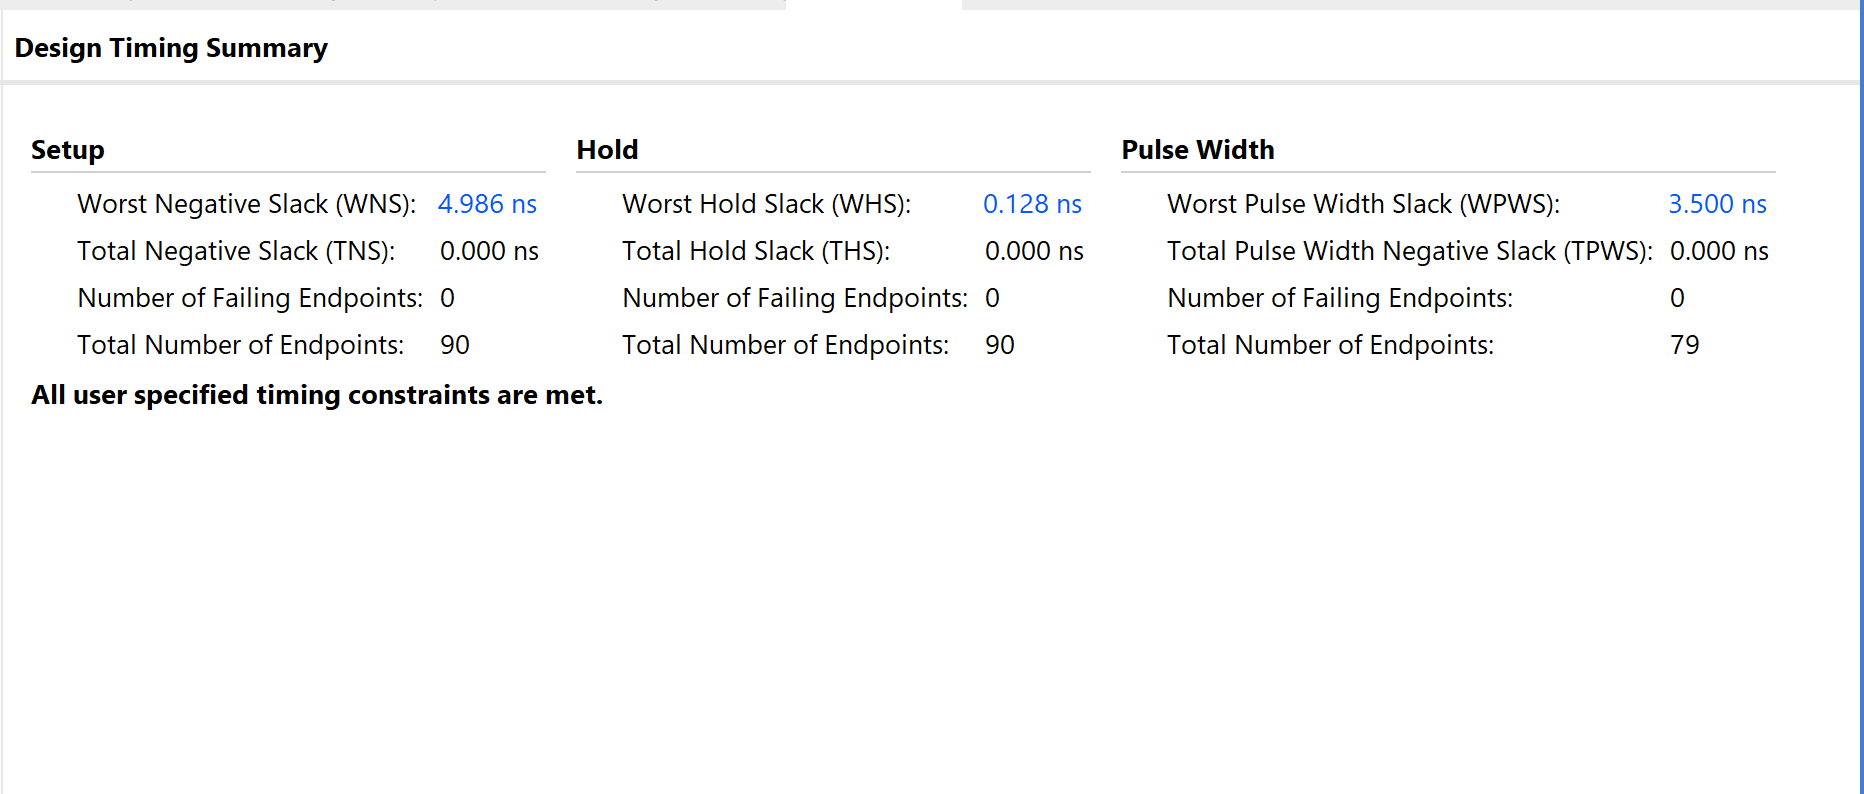
\includegraphics[width=1\linewidth]{graphics/result2.png}
    \caption{Post-Implementation Timing Summary}
\end{figure}

\begin{figure}[H]
    \centering
    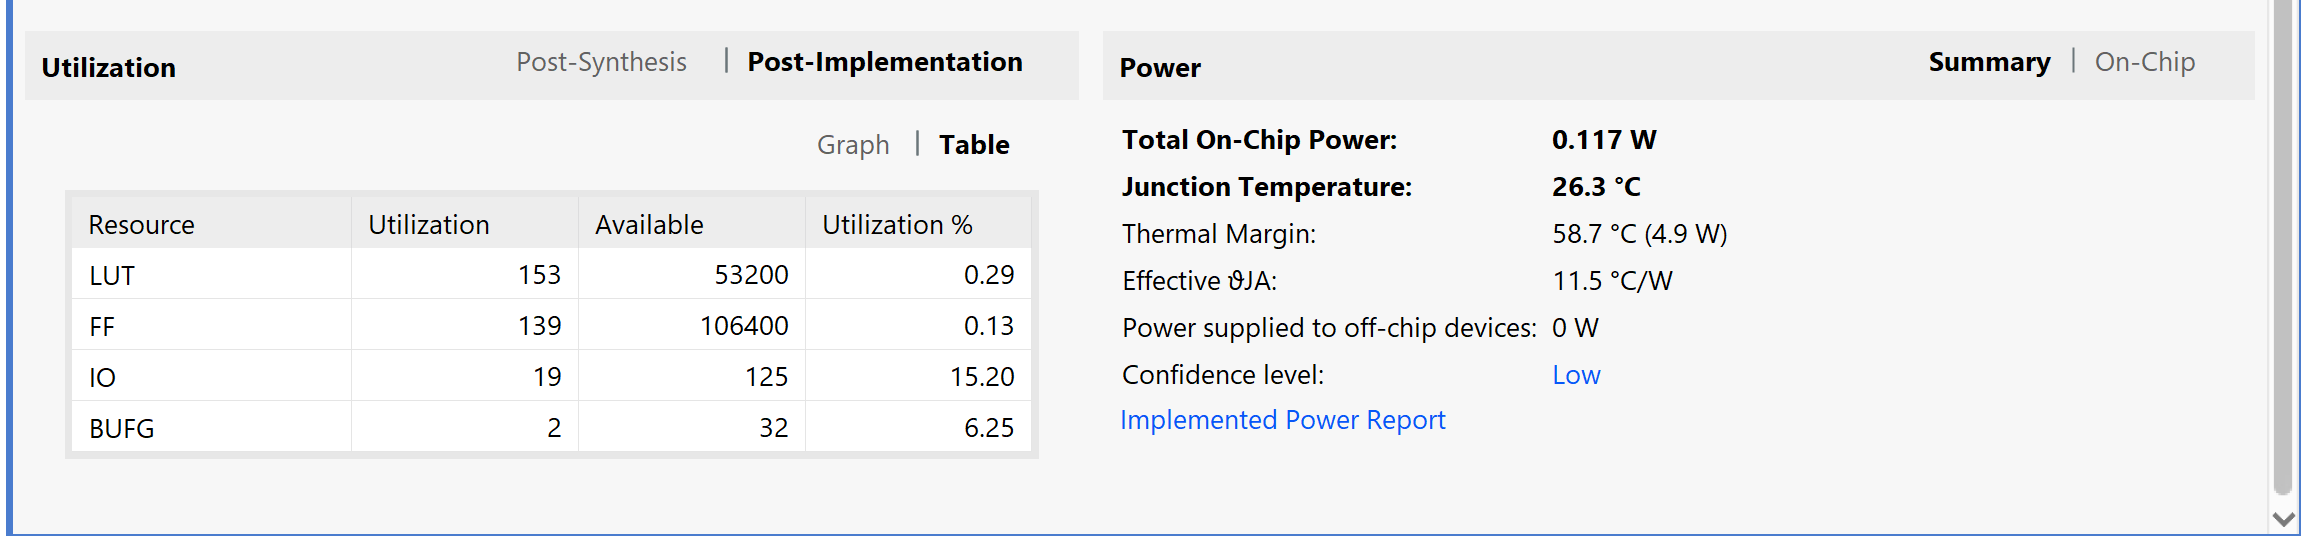
\includegraphics[width=1\linewidth]{graphics/result1.png}
    \caption{Post-Implementation Power Summary and Resource Utilization}
\end{figure}

\subsection{Resource Utilization}

The design uses very few FPGA resources:

\begin{table}[H]
\centering
\renewcommand{\arraystretch}{1.2}
\begin{tabular}{lrrrr}
\toprule
\textbf{Resource} & \textbf{Used} & \textbf{Available} & \textbf{Utilization (\%)} \\
\midrule
LUT  & 153 & 53,200  & 0.29\% \\
FF   & 139 & 106,400 & 0.13\% \\
IO   & 19  & 125     & 15.20\% \\
BUFG & 2   & 32      & 6.25\% \\
\bottomrule
\end{tabular}
\caption{Post-Implementation Resource Utilization}
\end{table}

\subsection{Power Analysis}

Vivado estimates the total on-chip power at 0.117 W, with a junction temperature of 26.3 \textdegree C and a thermal margin of 58.7 \textdegree C.

\begin{table}[H]
\centering
\renewcommand{\arraystretch}{1.2}
\begin{tabular}{ll}
\toprule
\textbf{Metric} & \textbf{Value} \\
\midrule
Total On-Chip Power & 0.117 W \\
Junction Temperature & 26.3 \textdegree C \\
Thermal Margin & 58.7 \textdegree C \\
Effective $\theta_{JA}$ & 11.5 \textdegree C/W \\
\bottomrule
\end{tabular}
\caption{Power Summary}
\end{table}

\subsection{Timing Analysis}

The design meets all timing constraints at an 8 ns clock period. The worst setup slack is 4.986 ns, the worst hold slack is 0.128 ns, and the worst pulse width slack is 3.500 ns.

\begin{table}[H]
\centering
\renewcommand{\arraystretch}{1.2}
\begin{tabular}{lcccc}
\toprule
\textbf{Metric} & \textbf{Setup} & \textbf{Hold} & \textbf{Pulse Width} \\
\midrule
Worst Slack (ns) & 4.986 & 0.128 & 3.500 \\
Failing Endpoints & 0 & 0 & 0 \\
\bottomrule
\end{tabular}
\caption{Timing Summary}
\end{table}

\subsection{Conclusion}

The implementation is compact, power-efficient, and fully meets timing requirements. With all constraints satisfied and low resource usage, the design is suitable for deployment and further extension.